\section{2020-02-07}
\underline{Roadmap}:
\begin{itemize}
    \item PPDAC example
    \item Interval estimation
          \begin{itemize}
              \item Intervals using the likelihood function
              \item Confidence intervals
          \end{itemize}
\end{itemize}
\underline{PPDAC}
\begin{itemize}
    \item Problem
    \item Plan
    \item Data
    \item Analysis
    \item Conclusion
\end{itemize}
\underline{Problem}
\begin{itemize}
    \item What kind of study is this?
          \begin{itemize}
              \item Observational
              \item Experimental
          \end{itemize}
    \item What kind of problem is this?
          \begin{itemize}
              \item Descriptive
              \item Causative
              \item Predictive
          \end{itemize}
    \item What is the target population?
          \begin{itemize}
              \item Target population: Population of interest
          \end{itemize}
    \item What are the variates and attributes of interest?
          \begin{itemize}
              \item Attribute $ = $ function of the variate of interest
              \item $ \theta= $ proportion of Canadians who believe climate change is the number one issue
          \end{itemize}
    \item What is the study population?
          \begin{itemize}
              \item Study population: The act of observing from which the sample is drawn
          \end{itemize}
    \item What is the sampling protocol?
          \begin{itemize}
              \item How is the sample collected?
          \end{itemize}
    \item What could be a source of study error?
    \item What could be a source of sampling error?
\end{itemize}
\underline{Analysis}

\underline{Data}: Try to avoid \textbf{bias} where bias is systematic error.

Blind study: \underline{Medical tests}
\begin{itemize}
    \item Control group $ \rightarrow $ Placebo (sugar pill)
    \item Experimental group $ \rightarrow $ Actual drug
    \item The patient does not know.
\end{itemize}
Double blind study: the doctors do not know

\underline{Types of errors}
\begin{itemize}
    \item Study errors: the difference in the value of the attribute between
          the target population and the study population
          \begin{itemize}
              \item $ \phi= $ proportion of people in Kitchener-Waterloo area who
                    believe climate change is the number one issue: $ \theta-\phi $
          \end{itemize}
    \item Sampling errors: the difference in value of the attribute between the study
          population and the sample: $ \phi-\hat{\pi} $ where $ \hat{\pi}= $
          sample proportion
    \item Measurement errors: the value of the variate vs what is actually recorded
          in the data
\end{itemize}
\underline{Conclusion}: Non-mathematical discussion of the final result

\underline{Interval estimation}

\underline{Objective}:
\begin{itemize}
    \item To find the ``reasonable'' values of $ \theta $, given by data set
    \item To quantify the ``reasonableness'' of your constructed interval
\end{itemize}
\underline{Method 1}: Through the likelihood function (likelihood interval)
\begin{defbox}
    \begin{definition}
        The $ 100p\% $ likelihood interval where $ p\in[0,1] $, is given by
        \[ \left\{ \theta:R(\theta)\geqslant p\right\} \]
        where $ R(\theta)= $ relative likelihood function.
    \end{definition}
\end{defbox}
\begin{exbox}
    \begin{example}
        Find the $ 10\% $ likelihood interval given the figure below.
        \begin{center}
            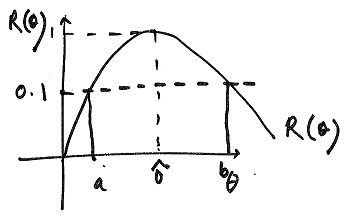
\includegraphics{likelihood interval.png}
        \end{center}
    \end{example}
\end{exbox}
\begin{center}
    \underline{Guidelines for Interpreting Likelihood Intervals}
\end{center}
\begin{center}
    \begin{tabular}{|c|}
        \hline
        Values of $ \theta $ inside a $ 50\% $ likelihood interval are very plausible in light of
        the observed data. \\
        \hline
        Values of $ \theta $ inside a $ 10\% $ likelihood interval are plausible in light of
        the observed data. \\
        \hline
        Values of $ \theta $ outside a $ 10\% $ likelihood interval are implausible in light of
        the observed data. \\
        \hline
        Values of $ \theta $ outside a $ 1\% $ likelihood interval are very implausible in light of
        the observed data. \\
        \hline
    \end{tabular}
\end{center}
\underline{Clicker Question 1}: THE MLE $ \hat{\theta} $ is in every likelihood
interval for all $ p\in[0,1] $.
\begin{enumerate}[label=(\alph*)]
    \item \textbf{True}
    \item False
\end{enumerate}
\underline{Clicker Question 2}: If $ \theta $ is in the $ p\% $ likelihood
interval, it has to be in the $ q\% $ likelihood interval if $ q>p $.
\begin{enumerate}[label=(\alph*)]
    \item True
    \item \textbf{False}
\end{enumerate}
